\lhead{\bfseries PERCEPTION}


\section*{Literature review}

Lane detection remains a cornerstone within the realm of advanced driver assistance systems, representing a critical element for intelligent autonomous systems and applications in smart vehicles. Notably, Lane Departure Warning Systems (LDWS) emerge as indispensable safety mechanisms, serving to alert drivers when their vehicles deviate from designated lanes on highways~\cite{choi2016advanced}. Over recent years, lane detection methodologies have undergone extensive scrutiny, leading to a classification of current studies into three primary categories: feature-based methods~\cite{suddamalla2015novel},~\cite{sehestedt2007robust},~\cite{liu2013lane}, model-based approaches ~\cite{wang2010model},~\cite{wang2004lane}, and deep learning techniques~\cite{kim2014robust},~\cite{zou2019robust}.

Feature-based methodologies typically entail the recognition of lanes through the analysis of lane marking attributes such as color and line edges. In this case, the input images are normally processed with contrast enhancement and edge detection techniques; after that, the lane markings in the image can be detected using a thresholding method, HT~\cite{albanesi1991time} or its variants (i.e., Randomized HT~\cite{mongkonyong2018lane}). However, a notable drawback of feature-based methods lies in their dependency on clearly delineated lane marks, rendering them susceptible to disruptions such as weak lane markings and occlusions. To address these limitations, the concept of Inverse Projection Mapping (IPM) has been introduced~\cite{Borkar2012}. By generating a bird's-eye view of the road surface, IPM circumvents issues associated with obscured or faint lane markings, although its efficacy relies heavily on the assumption of a perfectly flat road surface and precise camera calibration.

In model-based methods, lane markings are identified through the modeling of lanes using predetermined models such as straight-line, parabolic, or spline models. Various algorithms have been proposed, including combinations of Dynamic Programming (DP) and Hough Transform~\cite{wang2010model}, as well as curve model fitting methods in conjunction with gradient enhancement and edge detection techniques~\cite{Yoo2013}. However, the complexity of developing reliable models poses a significant challenge for model-based approaches.

Deep learning techniques, on the other hand, leverage deep learning algorithms, particularly Artificial Neural Networks (ANNs), to extract lane information. These methods, exemplified by the integration of Convolutional Neural Networks (CNNs) with algorithms like RANdom SAmple Consensus (RANSAC)~\cite{kim2014robust} or Recurrent Neural Networks (RNNs)~\cite{zou2019robust}, demonstrate promising capabilities in noise reduction and robust lane detection, especially in scenarios with challenging conditions such as bad lane markings or vehicle occlusion.

Despite their efficacy, the aforementioned state-of-the-art methods often entail high computational demands, particularly deep learning approaches. In response, this work proposes a novel Lane Detection algorithm based on Iterative Tree Search (ITS), designed specifically for low-cost hardware deployment. Characterized by its speed, computational efficiency, and low power consumption, the ITS-based approach represents a significant contribution to the field, offering a promising alternative to existing methodologies. Notably, to the best of our knowledge, there are no other algorithms for lane detection based on Iterative Tree Search, further highlighting the novelty and potential impact of this research endeavor.


Path following constitutes a significant application challenge within the domain of Unmanned Aerial Vehicles (UAVs), holding particular relevance in precision agriculture settings where robust path following algorithms are essential for maintaining high productivity rates and facilitating optimal plant growth~\cite{1_basso2019uav}. Moreover, in civilian applications such as power line monitoring, path following encapsulates the essential task of navigating between multiple target regions requiring inspection~\cite{Silano2021ICRARAL}. Irrespective of the specific application domain, the successful completion of missions by drones hinges upon their ability to safely and accurately follow predefined paths.

Examining the path following problem reveals two distinct components: path detection and path following~\cite{Dahroug2018MARSS, Rafique2020TAES}. In terms of path detection, the Hough transform and its advancements are widely regarded as prominent solutions in the literature s~\cite{6_duan2010improved, Du2010TIMP,5_duda1972use}. However, the computational demands associated with such transformations pose challenges, particularly for on-board implementation in aircraft with stringent battery and processing constraints. These challenges are further exacerbated in the context of Micro Aerial Vehicles (MAVs) where both sensor equipment and vehicle dimensions are minimal. Conversely, lightweight machine learning solutions have emerged as promising alternatives for path detection, albeit the time required for algorithm setup impedes their practical application in real-world scenarios~\cite{7_van2019ls, Tang2021PR}. Hence, there is a growing interest in low computational intensity algorithms capable of providing path following references within predefined time constraints, even without prior knowledge of the surrounding environment.

Transitioning to the path following stage, much of the state-of-the-art solutions~\cite{8_sujit2013evaluation, 12_pelizer2017comparison} rely on the use of nonlinear guidance laws~\cite{Keshmiri2018ICUAS}, vector fields~\cite{Tuttle2021ARC}, and pure pursuit algorithms owing to their simplicity and ease of implementation~\cite{Baqir2020IOP}. While the choice of path planner is contingent upon specific application requirements, certain general considerations can be made. Nonlinear guidance laws, while simple to implement, exhibit degraded performance in scenarios characterized by rapid changes in target acceleration, leading to significant trajectory generation delays and instability~\cite{Keshmiri2018ICUAS}. Consequently, ensuring stability necessitates a comprehensive understanding of target velocity and acceleration dynamics. Conversely, while vector field solutions mitigate oscillation issues inherent in nonlinear guidance laws, they entail substantial computational overhead which is not suitable for embedded systems present on a UAV~\cite{Tuttle2021ARC}. Meanwhile, the pure pursuit approach offers a viable solution for scenarios where tracking accuracy and computational efficiency are paramount. By dynamically adjusting the position of a look-ahead point based on predefined tracking criteria, pure pursuit algorithms aim to minimize the distance between the current position and the anticipated path, thereby facilitating precise path following~\cite{Gautam2015ICUAS, 10_xavier2019path, Silano2019SMC}.



\chapter{Enhanced Vision-Based UAV Path Following Strategy}
\label{Chapter:1}


In this chapter, we embark on an exploration of a novel algorithm designed for unmanned aerial vehicles (UAVs), focusing particularly on the path following and landing accuracy challenges that are pivotal in autonomous flight operations. The emergence of UAVs has revolutionized numerous sectors, including surveillance, delivery services, and environmental monitoring, by offering unprecedented flexibility and access to remote areas. However, the full potential of UAVs is contingent upon the advancement of robust navigation and control algorithms that can ensure precise maneuvering and operational reliability in diverse environments.

This research delves into the development and validation of an innovative algorithm that synergizes the pure pursuit path tracking methodology with advanced image processing techniques. This integration is tailored to enhance path detection and adherence capabilities, enabling UAVs to navigate and complete missions with heightened accuracy and efficiency. The motivation behind this algorithm springs from the need to address the computational constraints of micro aerial vehicles (MAVs), which necessitate lightweight yet effective solutions for real-time path following and target landing tasks.

The chapter sets the stage by outlining the theoretical underpinnings of the pure pursuit algorithm and its adaptation to the unique dynamics of UAV flight. It further discusses the incorporation of image processing for dynamic path detection, a critical component for ensuring the UAV's adaptability to varying operational scenarios. The mathematical models and simulation frameworks employed to evaluate the algorithm's performance are introduced, providing a foundation for the subsequent analysis of numerical results.

A significant highlight of this research is its practical validation through participation in the IFAC2020 MathWorks Minidrone competition, a prestigious event that challenges participants to demonstrate the efficacy of their control algorithms in real-world scenarios. This competition not only serves as a rigorous testing ground for the algorithm but also as a benchmark for its success against international standards.

By offering an open-source implementation of the algorithm, this chapter contributes to the broader UAV research community, facilitating further exploration, adaptation, and enhancement of path following techniques. The introduction sets the tone for a detailed investigation into the algorithm's development, its operational merits, and its triumphant validation in a competitive arena, underscoring its potential to redefine UAV navigation and control paradigms.

\newpage




\section{Problem Description}
\label{sec:problemDescription}

The work presented here finds an application within the IFAC2020 MathWorks Minidrone competition~\cite{4_Mathworks_url}, where the use of a model-based design approach is the aim of the specific contest. Path error and mission time are used as evaluation metrics for the algorithm. The whole process is the following: a quad-rotor~\gls{UAV} follows a pre-established red path by using its downward facing camera to get feedback from the environment. Images are updated according to the position and orientation of the vehicle simulated in the MATLAB~\gls{VR} world. No prior knowledge on the path and the surrounding scenario is given. The drone takes off and starts its motion looking at the path, and the mission stops with the recognition of an end-marker. At that time, the drone lands staying within the delimited area. Figure~\ref{fig:arena} shows the considered scenario. 
%
\begin{figure}[h]
	\centering
	\begin{tikzpicture}
		\node[anchor=south west,inner sep=0] (img) at (0,0) { 
			\includegraphics[width=0.45\textwidth]{figure/Part1/Chapter3/figures/track.png}};
		\begin{scope}[x={(img.south east)},y={(img.north west)}]
			
			% Solid circles for the drones, from left to right
			\draw [white, dashed, ultra thick] (0.95, 0.48) circle (0.065);
			
		\end{scope}
	\end{tikzpicture}
	\caption{Snapshot extracted from the virtual scenario. A dashed circle is used to indicated the drone position.}
	\label{fig:arena}
\end{figure}

\section{Vision-Based Path Following Algorithm}
\label{sec:purPursuitTrackingAlgorithm}


The vision-based path following algorithm combines the advantages offered by the pure pursuit algorithm~\cite{14_coulter1992implementation} with that of an easy image processing system to cope with the task. The algorithm starts selecting a target position ahead of the vehicle and that has to be reached, typically on a path. The framework is based on the following operations: (i) given the actual position $\mathbf{d}=(x_d, y_d)^\top \in \mathbb{R}^2$ where the~\gls{UAV} is located, a~\gls{VTP} is set over the track at $\mathbf{w}=(x_w, y_w)^\top \in \mathbb{R}^2$; then, (ii) the quad-rotor is commanded to reach the~\gls{VTP} along a straight line (essentially it is the pure pursuit algorithm with a curvature of infinite radius)~\cite{14_coulter1992implementation}, i.e., moving the vehicle from its current position to the goal position\footnote{The quad-rotor is assumed to fly at a fixed height along the entire mission.}. In Figure~\ref{fig:pure pursuit} an illustrative example of how the algorithm works is depicted. 

\begin{figure}
	\centering
	\includegraphics[scale=0.75]{figure/Part1/Chapter3/figures/purepursuit.png}
	\caption{An illustrative example of the proposed vision-based path following algorithm works. The red point $\mathbf{d}$ represents the drone position, while the orange point $\mathbf{w}$ depicts the~\gls{VTP}.}
	\label{fig:pure pursuit}
\end{figure}

Contrary to the pure pursuit algorithm, the proposed approach exploits the intrinsic characteristics of the multi-rotor~\glspl{UAV} motion: differently from ground vehicles with steering wheels, drones can follow a path without modifying their heading. Such an assumption allows reducing the time to accomplish the task by removing the control of the heading from the purposes of the path follower. %The testing of the algorithm is performed inside a Simulink virtual scenario, where a path is created as shown in Figure~\ref{fig:arena}. 

In Figure~\ref{fig:block diagram} the whole control scheme architecture is reported. The algorithm is mainly divided into two parts: (i) the~\gls{IPS} deals with extracting the red path from the camera images, providing the errors along the $x$- and $y$-axis of the camera frame between the current drone position and the~\gls{VTP} point, and recognizing the End-Marker for the landing operations; while, (ii) the~\gls{PP} figures out the path following problem by computing the new position $\mathbf{w}$ of the drone in the world frame\cite[Sec.~V]{SilanoMATFly} implementing an~\gls{IBVS} scheme. The control algorithm computes the commands $u_T$, $u_\varphi$, $u_\vartheta$, and $u_\psi$ that should be given to the drone in order to update its position and orientation in accordance to the~\gls{PP} references. 

\begin{figure}
	\begin{center}
		\scalebox{1.2}{
			\begin{tikzpicture}
				
				%%%%%%%%%%%%%%%%% Node - Image Processing System
				\node (ImageProcessingSystem) at (-1.5,0) [draw, rectangle, minimum width=2cm, minimum 
				height=1cm, text centered, text width=5em]{Image Processing};
				
				% Curly brackets
				\draw [decorate,decoration={brace, mirror, amplitude=10pt,raise=4pt},yshift=0pt] 
				(-2.5,-0.5) -- (-0.5,-0.5) node [black,midway,xshift=0.0cm,yshift=-0.8cm] {Sec.~III-A};
				
				%%%%%%%%%%%%%%%%% Node - Path Planner
				\node (PathPlanner) at (1.25,0) [draw, rectangle, minimum width=2cm, minimum 
				height=1cm, text centered, text width=5em]{Path Planner};
				
				% Curly brackets
				\draw [decorate,decoration={brace, mirror, amplitude=10pt,raise=4pt},yshift=0pt] 
				(0.25,-0.5) -- (2.25,-0.5) node [black,midway,xshift=0.0cm,yshift=-0.8cm] {Sec.~III-B};
				
				%%%%%%%%%%%%%%%%% Node - Controller
				\node (Controller) at (4.00,0) [draw, rectangle, minimum width=2cm, minimum height=1cm, 
				text centered, text width=5em]{Controller};
				
				%%%%%%%%%%%%%%%%% Node - Drone
				\node (Drone) at (7.15,0) [draw, rectangle, minimum width=2cm, minimum height=1cm, text 
				centered, text width=5em]{Drone};
				
				% Curly brackets
				\draw [decorate,decoration={brace, mirror, amplitude=10pt,raise=4pt},yshift=0pt] 
				(3.00,-0.5) -- (8.15,-0.5) node [black,midway,xshift=0.0cm,yshift=-0.8cm] {Competition Organizers};
				
				% Links
				\draw[-latex] (ImageProcessingSystem) -- node[above]{$e_x$} node[below]{$e_y$} (PathPlanner);
				\draw[-latex] (PathPlanner) -- node[above]{$x_w$} node[below]{$y_w$} (Controller);
				\draw[-latex] (Controller) -- node[above]{$u_T$, $u_\varphi$} node[below]{$u_\vartheta$, $u_\psi$} (Drone);
				\draw[-latex] (Drone) -- ($ (Drone) + (1.5,0)$) -- ($ (Drone) + (1.5,-2.5)$) -- ($ 
				(ImageProcessingSystem) - (1.5,2.5)$) -- ($ (ImageProcessingSystem) - (1.5,0)$) --  
				(ImageProcessingSystem);
				
				% Text
				\node at ($ (PathPlanner) - (-1.5,2.45)$) [text centered, above]{IMG};
				
			\end{tikzpicture}
		}
	\end{center}
	\caption{Control system architecture. From left to right: the image processing, path planner, controller, and drone blocks.}
	\label{fig:block diagram}
\end{figure}

The overall mission is divided into four parts: \textit{Take off}, \textit{Following}, \textit{End-Marker}, and \textit{Landing}. A decision-making process has been implemented to achieve the competition objectives triggering the system from a state to another, as depicted in Figure~\ref{fig:state machine}. For each frame, the~\gls{IPS} accesses the system status and plan the next action (i.e., landing, following, etc.). The drone starts taking off from its initial position looking at the path. Once the vehicle reaches the hovering position, the~\gls{IPS} detects the path and the state machine enters in the \textit{Following} state, hence the path following starts. As soon as the~\gls{IPS} detects the End-Marker, the state machine exits from the \textit{Following} state and goes into the \textit{End-Marker} state. At this stage the mission stops, and the drone starts the landing. In the following subsections the implementation of the image processing system and path planner modules are detailed.
%
\begin{figure}
	\centering
	\begin{tikzpicture}[->, >=stealth', shorten >=0.8pt, auto, semithick, initial text=${\rm start}$]
		
		\tikzstyle{every state}=[fill=white,text=black]
		
		\node[initial,state] (A)                    {$1$};
		\node[state]         (B)        [ right= 4cm of A] {$2$};
		\node[state]         (C) [ below= 2cm of B] {$3$};
		\node[accepting,state](D) [ left= 4cm of C] {$4$};
		
		\path (A) edge              node {${ \rm Hovering} \wedge {\rm Flag\_VTP}$} (B)
		edge [loop above] node {{${ \rm \overline{Hovering}}$}} (A)
		(B) edge       [left]       node {${ \rm \overline{Flag\_VTP} \wedge Flag\_marker}$} (C)
		edge [loop above] node {${ \rm Flag\_VTP}$} (B)
		(C) edge              node {${\rm Centered}$} (D)
		edge [loop below] node {${ \rm \overline{Centered}}$} (C);
		
	\end{tikzpicture}
	\caption{State machine implemented. State 1: \textit{Take-off}. State 2: \textit{Following}. State 
		3: \textit{End-Marker}. State 4: \textit{Landing}.} 
	\label{fig:state machine}
\end{figure} 


\subsection{Image processing system}
\label{sec:imageProcessingSystem}

Starting from the camera frames, the~\gls{IPS} takes care of separating the features of the pre-established path from that of the environment. % The main objective of the module is in the detection, especially track  and landing mark detection in the \textit{Track} and \textit{End-Marker} phases, respectively. Moreover, the~\ac{IPS} is in charge of triggering the state machine from a state to another and to handle the decision-making process during the competition mission.

The~\gls{IPS} receives frames of width $W$ and height $H$ from the camera sensor at each   $T_\mathrm{IPS} = \SI{0.2}{\second}$, i.e., the camera sampling time. The image format is RGB with $8$ bits for each color channel. The path is \SI{0.01}{\meter} in width, while the landing marker is circular with a diameter of \SI{0.02}{\meter}. The path color is red, and this information is taken into consideration in all the elaborations to filter out the background scenario. The procedure consists of the following steps: first, the RGB frame is converted into an intensity level frame representation as follows 
%
\begin{equation}
	F(n,m)=f_R(n,m) -  \frac{f_G(n,m)}{GG} - \frac{f_B(n,m)}{GB} ,
\end{equation}
%
where the pair $(n,m)$ represents the pixel located at row $n \in \{1, 2, \dots, H\}$ and column $m \in \{1, 2, \dots, W\}$ of the image frame and $f_i$, with $i \in \{R, G, B\}$, provides the intensity level representation of the corresponding red, green and blue channels. An heuristic approach was used to tune the $GG$, $GB \geq 1$ parameter values. These parameters help to detect the pixels belonging to the path. Further, a binarization process based on a $K_T$  threshold value refines the process removing artifacts from the elaboration. The binarized frame can be described by the binary function $F_\mathrm{bin} \colon (n,m) \to \{0, 1\}$ whose output is one when the pixel belongs to the path and zero otherwise. Finally, an erosion operation is performed through a square kernel to shrink and regularize the binarized frame. In Figure~\ref{fig:preprocessing} the overall process is reported for a single sample frame.

\begin{figure}
	\centering
	\includegraphics[width=0.75\textwidth]{figure/Part1/Chapter3/figures/bin_ero_track.jpg}
	\caption{Original frame (upper left),  converted and binarized frame (upper right), and eroded frame (lower).}
	\label{fig:preprocessing}
\end{figure}

Then, the obtained reference path is used in a twofold way: (i) to identify a new~\gls{VTP} belonging to the track; (ii) to detect the landing marker. The two tasks are described in the pseudocode reported in Algorithm~\ref{alg:imageProcessing}.

Looking at the algorithm, the first three functions (i.e., \texttt{channelConv}, \texttt{binarization}, and \texttt{erosion}) take care of extracting the path information from the frame. Then, the \texttt{detectTrack} and \texttt{detectMarker} functions deal with raising a flag when the path (\texttt{Flag\_VTP}) or the End-Marker (\texttt{Flag\_marker}) are detected. The path following algorithm starts with the~\gls{IPS} that computes the errors ($e_x$ and $e_y$) between the drone position and the~\gls{VTP} point for the~\gls{PP} by using a circular arc mask centered in the drone~\gls{CoM}\footnote{The assumption that the~\gls{CoM} being in the center of the reference frame, i.e., $x_\mathrm{CoM} = \frac{H}{2}$ and $y_\mathrm{CoM}=\frac{W}{2}$, is taken into consideration.} with thickness $R_\mathrm{max} - R_\mathrm{min}$\footnote{$R_\mathrm{max}$ and $R_\mathrm{min}$ are the outer and inner radius, respectively.}. 
%
% FOR ALGORITHM UAV
\def\BState{\State\hskip-\ALG@thistlm}
%
\begin{algorithm}
	\caption{Image Processing System}\label{alg:imageProcessing}
	\begin{algorithmic}[1]
		\State $\text{IMG}  \gets \text{channelConv(\text{IMG})}$, \\
		$\text{IMG} \gets \text{binarization(\text{IMG})}$, \\
		$\text{IMG} \gets \text{erosion(\text{IMG})}$, \\
		$\text{Flag\_VTP} \gets \text{detectTrack(\text{IMG})}$, \\
		$\text{Flag\_marker}$ $\gets \text{detectMarker(\text{IMG})}$
		
		\If {$\text{Flag\_VTP}$} \\ 
		\quad $x_\mathrm{VTP}$, $y_\mathrm{VTP} \gets \text{vtp(frame)}$ \\
		\quad $e_x \gets x_\mathrm{VTP} - x_\mathrm{CoM}$ \\
		\quad $e_y \gets y_\mathrm{VTP} - y_\mathrm{CoM}$
		\Else \If{$\text{Flag\_marker}$} \\
		\quad \quad $\;$ $x_\mathrm{MARK}$, $y_\mathrm{MARK} \gets \text{cgMarker(frame)}$ \\
		\quad \quad $\;$ $e_x \gets x_\mathrm{MARK} - x_\mathrm{CoM}$ \\ 
		\quad \quad $\;$ $e_y \gets y_{\rm MARK} - y_{\rm CoM}$
		\EndIf \EndIf
		
		\State \Return $e_x$, $e_y$, $\text{Flag\_VTP}, \text{Flag\_marker}$ 
	\end{algorithmic}
\end{algorithm}


In Figure~\ref{fig:Arc_mask}, the arc mask considering the~\gls{VTP} position at time $\mathbf{t}_k$ is depicted, where $\mathbf{t}_k$ denotes the $k$-element of the time interval vector defined as $\mathbf{t} =(0, T_\mathrm{IPS}, \dots, NT_\mathrm{IPS})^\top \in \mathbb{R}^{N+1}$, with $k \in \mathbb{N}_0$. The orientation angle \mbox{$\vartheta = \arctantwo(x_\mathrm{VTP},y_\mathrm{VTP})$} is calculated with respect to the frame coordinates, where the $\arctantwo$ function is the four-quadrant inverse of the tangent function. A portion~$\varTheta$ of the arc mask is established by taking into account the previous~\gls{VTP}'s orientation. In particular, we set up two semi-arcs with width~$\frac{\varTheta}{2}$, namely~\gls{FOV}, in counter-clockwise and clockwise directions from $\vartheta$. Then, the arc mask is applied to the eroded image obtaining the~\gls{VTP} point at $\mathbf{t}_{k+1}$. The function~\gls{VTP} calculates $x_\mathrm{VTP}$, $y_\mathrm{VTP}$, and $\vartheta$ which represent the frame coordinates and angle orientation of the~\gls{VTP} at  $\mathbf{t}_{k+1}$, respectively. Subsequently the corresponding errors with respect to the center of mass, i.e., $e_x$ and $e_y$, are computed inside the frame coordinates. Finally, the \texttt{Flag\_VTP} and the $e_x$ and $e_y$ values are provided as input to the~\gls{PP} at each $T_\mathrm{IPS}$. Figure~\ref{fig:track} shows the result of the entire process setup. 

\begin{figure}
	\begin{center}
		\scalebox{1.65}{
			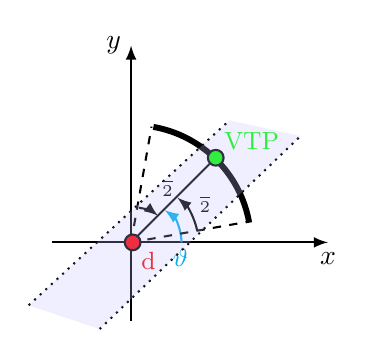
\begin{tikzpicture}
				
				% Axes of the image frame
				\draw[-latex] (-1.00,0) -- (2.5,0) node[below]{$x$};
				\draw[-latex] (0,-1.0) -- (0,2.5) node[left]{$y$};
				
				% Circle of the circular mask
				\draw[line width=2.15pt] (1.5,0.25) arc(10:80:1.5);
				
				% Radius
				\draw[-] (0,0) -- (1.05,1.05);
				%\node at (0.75,0.75) [left]{\scriptsize $R_\mathrm{min}$};
				%\node at (1.25,1.45) [left]{\scriptsize $R_\mathrm{max}$};
				
				% Length errors
				%\draw[green,-, line width=1.25pt] (0,0) -- node[above left]{\small $e_y$} (0,1.04);
				%\draw[blue,-, line width=1.25pt] (0,0) -- node[below right]{\small $e_x$} (1,0);
				%\draw[dotted] (1,0) -- (1,1.04);
				%\draw[dotted] (0,1.04) -- (1,1.04);
				\draw (0,0) arc(0:20:0.3);
				\draw[-latex] (0.84,0.15) arc (12:50:0.75cm);
				\node at (0.70,0.75) [below right]{\small $\frac{\varTheta}{2}$}; % first angle
				\draw[-latex] (0.10,0.44) arc (82.5:52:0.5cm);
				\node at (0.70,0.70) [left]{\small $\frac{\varTheta}{2}$}; % second angle
				\draw[-latex, cyan] (0.64,0) arc (0:55:0.5cm);
				\node at (0.40,0.05) [below right, cyan]{\small $\vartheta$}; % first angle
				
				% End
				\draw[dashed] (0,0) -- (0.26,1.47); % cos(80)*1.5, sin(80)*1.5
				\draw[dashed] (0,0) -- (1.47,0.26); % cos(10)*1.5, sin(10)*1.5
				\draw[fill=red] (-0.08,0) arc(-180:180:0.1); % balls
				\node at (0,0) [below right]{\textcolor{red}{\small{d}}};
				\draw[fill=green] (0.975,1.075) arc(-180:180:0.1); % balls
				\draw (1.05, 1.05) node[above right]{\textcolor{green}{\small{VTP}}};
				
				% Adding path
				\draw[dotted] (-1.30, -0.80) -- (1.25,1.55);
				\draw[dotted] (-0.40, -1.10) -- (2.15,1.35);
				\fill[blue!25, nearly transparent] (-1.30, -0.80) -- (1.25,1.55) -- (2.15,1.35) -- 
				(-0.40, -1.10) -- cycle;
				
			\end{tikzpicture}
		}
	\end{center}
	\caption{Arc mask. The drone position (red), the previous~\gls{VTP} (green), and the pre-established path to follow (purple) are reported.} 
	\label{fig:Arc_mask}
\end{figure}
%
\begin{figure}
	\centering
	\includegraphics[width=0.75\textwidth]{figure/Part1/Chapter3/figures/VTP_Algorithm_1.png}
	\caption{Frame after the application of the Arc mask (left). Extracted pixels belonging to the path (right).}
	\label{fig:track}
\end{figure}

It is worth noticing that when the landing marker is detected and no other~\gls{VTP} point is found in the frame, the~\gls{IPS} triggers the state machine in the \texttt{End-Marker} state. Here, the new main task of the~\gls{IPS} is to obtain the position of the End-Marker within the frame coordinates. An additional erosion process is performed by using a circular kernel, as depicted in Figure~\ref{fig:End_marker}. 

\begin{figure}
	\centering
	\includegraphics[width=0.75\textwidth]{figure/Part1/Chapter3/figures/land_marker.png}
	\caption{Original (left) and eroded frames (right) of the End-Marker are reported.}
	\label{fig:End_marker}
\end{figure}

\subsection{Path planner}
\label{sec:pathPlanner}

The~\gls{PP} is designed to compute the position of the~\gls{VTP} point $\mathbf{w} = (x_w, y_w)^\top$ maintaining a constant altitude ($z_H$) while following the path. Roughly speaking, the~\gls{PP} computes the spatial coordinates $x_w$ and $y_w$ trying to reduce the errors, i.e., $e_x$ and $e_y$, between the drone position and the~\gls{VTP}. These values are later used by the drone controller to tune the command signals $u_T$, $u_\varphi$, $u_\vartheta$, and $u_\psi$, as described in Figure~\ref{fig:block diagram}. The proposed path planner is based on~\gls{PI} control loops. As a common rule in cascade structure, the inner loop, i.e., the~\gls{PP}, is regulated at a rate faster than the outer loop, i.e., the~\gls{IPS}. In our case, the~\gls{PP} runs at $\SI{200}{\hertz}$ ($T_\mathrm{PP} = \num{5e-3} \si{\second}$) while the~\gls{IPS} runs at $\SI{2}{\hertz}$ ($T_\mathrm{IPS} = \SI{0.2}{\second}$). These are a standard solution in the literature for quad-rotors control design~\cite{Dief2015}.

As described in Sec.~\ref{sec:purPursuitTrackingAlgorithm}, the path following stops with the detection of the End-Marker. At that time, the~\gls{IPS} implements a toggle switch behavior raising the \texttt{Flag\_marker} flag while holding low the \texttt{Flag\_VTP} flag. This mutually separates the \textit{Following} and \textit{Landing} phases avoiding instability issues. The pseudocode of the proposed algorithm is reported in Algorithm~\ref{alg:pathPlanner} with parameter values detailed in Table~\ref{tab:parameters}.

In Subsection~\ref{subsec:uavVelocity}, we show how $\alpha$ can be set to control the velocity of vehicle along the entire mission. Therefore, the proposed Vision-Based Path Following algorithm makes it possible not only to generate the spatial coordinates $x_w$ and $y_w$ using a~\gls{IBVS} scheme but also to set the velocity during the entire mission.

\begin{algorithm}
	\caption{Path Planner}\label{alg:pathPlanner}
	\begin{algorithmic}[1]
		\State $e_x$, $e_y$, $\text{Flag\_VTP}$, $\text{Flag\_marker}$ 
		
		\If{$\text{Flag\_VTP}$} \\
		\quad $x_{k+1} \gets x_k + \alpha e_x$\\
		\quad $y_{k+1} \gets y_k + \alpha e_y$\\
		\quad $z_{k+1} \gets  z_H$
		\EndIf
		
		\If{$\text{Flag\_marker}$}
		\If{$(e_x=0 \wedge e_y=0)$} \\
		\quad \quad $\;$ $x_{k+1}  \gets x_k $\\
		\quad \quad $\;$ $y_{k+1} \gets y_k $\\
		\quad \quad $\;$ $z_{k+1} \gets 0$
		\Else \\
		\quad \quad $\;$ $x_{k+1} \gets x_k + \beta e_x$\\
		\quad \quad $\;$ $y_{k+1}  \gets y_k + \beta e_y$\\
		\quad \quad $\;$ $z_{k+1} \gets z_H$
		\EndIf \EndIf
		
		\State $x_w \gets x_{k+1}$, $y_w \gets y_{k+1}$, $z_w \gets z_{k+1}$
		
		\State \Return $x_w$, $y_w$, $z_w$
	\end{algorithmic}
\end{algorithm} 

%The~\ac{PP} obtains the state position estimations every \mbox{$T_\mathrm{PP}=\SI{0.05}{\second}$}; consequently, it can plan a new position to reach according to its sampling time. The behavior of the PP depends on the state machine, there are two operating modes: one is implemented to track a~\ac{VTP} and the other one is employed to reach the central point of the End-Marker. The two dynamic behaviors differ from each other: the~\ac{PP} used to track a~\ac{VTP} has to produce a trajectory with a high velocity and a minimum error between the~\ac{CG} of the drone and the arena track. The control parameter $\alpha$ regulates the operating mode during the \textit{Track} phase, choosing high values allow to decrease the time to reach the~\ac{VTP}. During the \textit{End-Marker}, the drone has to reach the End-Marker position with a good accuracy avoiding to overtake it, for this reason the values of the control parameters $\beta$, which regulates this drone behavior during this phase, have to be low.

%%% END SECTION ============================================================

%%% START SECTION ==========================================================

\section{Numerical Results}
\label{sec:simulationsResults}

To demonstrate the validity and effectiveness of the proposed framework, numerical simulations have been carried out by using the 2019b release of MATLAB equipped with MathWorks Virtual Reality toolbox~\cite{16_Mathworks_url} and Parrot support package for Simulink~\cite{15_Mathworks_url}. The video available at~\cite{YouTubeVideo} illustrates in a direct way how the system works, i.e., the ability of the quad-rotor~\gls{UAV} to follow the pre-established red path and to land on the End-Marker. In addition, the video shows the behavior of the~\gls{IPS} and~\gls{PP} that never lose the path during the entire mission. 
%The testing of the algorithm is performed inside a Simulink virtual scenario, where a path is created as shown in Figure~\ref{fig:arena}. 

In Figure~\ref{fig:plot_trajectory} a comparison of the system performance by using various values of $\alpha$ is reported. As can be seen from the plots, the larger $\alpha$ is, the lower the mission time ($T_s$) is. On the other hand, the lower the mission time is, the greater the path error is. Looking at the zoom plot (see, Figure~\ref{subfig:comparisonPlot}) it is even clearer how the system performance degrades with increasing $\alpha$ value, and these are all the more evident as the path is angular. For the considered scenario, an heuristic approach was used to tune the $\alpha$ and $\beta$ parameter values.



\begin{figure}[t]
	\begin{center}
		\hspace{-0.725cm}
		\begin{subfigure}[c]{0.45\columnwidth}
			\scalebox{0.8}{
				\begin{tikzpicture}
					\begin{axis}[%
						width=2.8119in,%
						height=1.8183in,%
						at={(0.758in,0.481in)},%
						scale only axis,%
						xmin=-3.7,%
						xmax=0,%
						ymax=3,%
						ymin=-0.25,%
						xmajorgrids,%
						ymajorgrids,%
						ylabel style={yshift=0cm}, %shifting the y line text
						xlabel={X [\si{\meter}]},%
						ylabel={Y [\si{\meter}]},%
						axis background/.style={fill=white},%
						legend style={at={(0.725,0.875)},anchor=north,legend cell align=left, draw=none, 
							draw=white!15!black}
						]
						%
						\addplot [color=blue, solid, line width=1.15pt] 
						file{figure/Part1/Chapter3/matlabPlots/track_downsampled.txt};%
						%
						\addplot [color=red, dashed, line width=1.15pt] 
						file{figure/Part1/Chapter3/matlabPlots/alpha_005_downsampled.txt};%
						%
						\legend{$\text{path}$, $\alpha = 0.05\text{,}\, T_s = \SI{30}{\second}$};%
					\end{axis}
				\end{tikzpicture}
			}
			\caption{}
		\end{subfigure}
		%
		\hspace{0.25cm}
		%
		\begin{subfigure}[c]{0.45\columnwidth}
			\scalebox{0.8}{
				\begin{tikzpicture}
					\begin{axis}[%
						width=2.8119in,%
						height=1.8183in,%
						at={(0.758in,0.481in)},%
						scale only axis,%
						xmin=-3.7,%
						xmax=0,%
						ymax=3,%
						ymin=-0.25,%
						xmajorgrids,%
						ymajorgrids,%
						ylabel style={yshift=0cm}, %shifting the y line text
						xlabel={X [\si{\meter}]},%
						ylabel={Y [\si{\meter}]},%
						axis background/.style={fill=white},%
						legend style={at={(0.725,0.875)},anchor=north, legend cell align=left, draw=none, 
							draw=white!15!black}
						]
						%
						\addplot [color=blue, solid, line width=1.15pt] 
						file{figure/Part1/Chapter3/matlabPlots/track_downsampled.txt};%
						%
						\addplot [color=green, dashed, line width=1.15pt] 
						file{figure/Part1/Chapter3/matlabPlots/alpha_004_downsampled.txt};%
						%
						\legend{$\text{path}$, $\alpha = 0.04\text{,}\, T_s = \SI{34}{\second}$};%
					\end{axis}
				\end{tikzpicture}
			}
			\caption{}
		\end{subfigure}
		%
		\\
		\vspace{0.05cm}
		\hspace{-0.75cm}
		%
		\begin{subfigure}[c]{0.45\columnwidth}
			\scalebox{0.8}{
				\begin{tikzpicture}
					\begin{axis}[%
						width=2.8119in,%
						height=1.8183in,%
						at={(0.758in,0.481in)},%
						scale only axis,%
						xmin=-3.7,%
						xmax=0,%
						ymax=3,%
						ymin=-0.25,%
						xmajorgrids,%
						ymajorgrids,%
						ylabel style={yshift=0cm}, %shifting the y line text
						xlabel={X [\si{\meter}]},%
						ylabel={Y [\si{\meter}]},%
						axis background/.style={fill=white},%
						legend style={at={(0.725,0.875)},anchor=north,legend cell align=left, draw=none, draw=white!15!black}
						]
						%
						\addplot [color=blue, solid, line width=1.15pt] 
						file{figure/Part1/Chapter3/matlabPlots/track_downsampled.txt};%
						%
						\addplot [color=yellow, dashed, line width=1.15pt] 
						file{figure/Part1/Chapter3/matlabPlots/alpha_003_downsampled.txt};%
						%
						\legend{$\text{path}$, $\alpha = 0.03\text{,}\, T_s = \SI{47}{\second}$};%
					\end{axis}
				\end{tikzpicture}
			}
			\caption{}
		\end{subfigure}
		%
		\hspace{0.25cm}
		%
		\begin{subfigure}[c]{0.45\columnwidth}
			\scalebox{0.8}{
				\begin{tikzpicture}
					\begin{axis}[%
						width=2.8119in,%
						height=1.8183in,%
						at={(0.758in,0.481in)},%
						scale only axis,%
						xmin=-3.7,%
						xmax=-3.4,%
						ymax=3,%
						ymin=2,%
						xmajorgrids,%
						ymajorgrids,%
						ylabel style={yshift=0cm}, %shifting the y line text
						xlabel={X [\si{\meter}]},%
						ylabel={Y [\si{\meter}]},%
						axis background/.style={fill=white},%
						legend style={at={(0.475,0.945)},anchor=north,legend cell align=left, draw=none, legend columns=-1, draw=white!15!black}
						]
						%
						\addplot [color=red, dashed, line width=1.15pt] 
						file{figure/Part1/Chapter3/matlabPlots/alpha_005_downsampled.txt};%
						%
						\addplot [color=green, dashed, line width=1.15pt] 
						file{figure/Part1/Chapter3/matlabPlots/alpha_004_downsampled.txt};%
						%
						\addplot [color=yellow, dashed, line width=1.15pt] 
						file{figure/Part1/Chapter3/matlabPlots/alpha_003_downsampled.txt};%
						%
						\legend{$\alpha = 0.05$, $\alpha = 0.04$, $\alpha = 0.03$};%
						%
						\addplot [color=blue, solid, line width=1.15pt] 
						file{figure/Part1/Chapter3/matlabPlots/track_downsampled.txt};%
						%
					\end{axis}
				\end{tikzpicture}
			}
			\caption{}
			\label{subfig:comparisonPlot}
		\end{subfigure}
	\end{center}
	\caption{Trajectory plots. From left to right: the desired and the drone paths for various values of $\alpha$ are represented. The mission time $T_s$ and a comparison between the considered $\alpha$ values are also reported.}
	\label{fig:plot_trajectory}
\end{figure}

%\begin{figure}
%	\begin{center}
	%		\scalebox{1}{
		%			\begin{tikzpicture}
			%			\begin{axis}[%
				%			width=2.8119in,%
				%			height=1.8183in,%
				%			at={(0.758in,0.481in)},%
				%			scale only axis,%
				%			xmin=-3.7,%
				%			xmax=0,%
				%			ymax=3,%
				%			ymin=-0.25,%
				%			xmajorgrids,%
				%			ymajorgrids,%
				%			ylabel style={yshift=0cm}, %shifting the y line text
				%			xlabel={X [\si{\meter}]},%
				%			ylabel={Y [\si{\meter}]},%
				%			axis background/.style={fill=white},%
				%			legend style={at={(0.725,0.875)},anchor=north,legend cell 
					%				align=left,draw=none,draw=white!15!black}
				%			]
				%			%
				%			\addplot [color=blue, solid, line width=1.15pt] 
				%			file{matlabPlots/track_downsampled.txt};%
				%			%
				%			\addplot [color=red, dotted, line width=1.15pt, mark size=2, mark repeat=3, 
				%			mark=diamond*] file{matlabPlots/alpha_003_downsampled.txt};%
				%			%
				%			\addplot [color=green, dotted, line width=1.15pt, mark=x, mark size=2, mark repeat=3] 
				%			file{matlabPlots/alpha_004_downsampled.txt};%
				%			%
				%			\addplot [color=magenta, dotted, line width=1.15pt, mark=o, mark size=1, mark 
				%			repeat=3] file{matlabPlots/alpha_005_downsampled.txt};%
				%			%
				%			\legend{$\text{track}$, $\alpha = 0.03\text{,}\, T_s = \SI{47}{\second}$, $\alpha = 
					%			0.04\text{,}\, T_s = \SI{34}{\second}$, $\alpha = 0.05\text{,}\, T_s = 
					%			\SI{30}{\second}$};%
				%			\end{axis}
			%			\end{tikzpicture}
		%		}
	%	\end{center}
%	\caption{Trajectory plot. The desired and the drone paths for various $\alpha$ are represented. 
	%	The mission time $T_s$ is also reported.}
%	\label{fig:plot_trajectory}
%\end{figure}

Figure~\ref{fig:plot_velocity} depicts the drone velocity $v_x$ and $v_y$ along the $x$- and $y$-axis, respectively, and the norm of the drone velocity $v_D$. As described in Sec.~\ref{sec:pathPlanner} and detailed in~\ref{subsec:uavVelocity}, the norm of the drone velocity remains approximately constant while following the path. The presence of spikes might be due to the coupling effects of the drone $xy$ dynamics even though $x_w$ and $y_w$ references have not been modified yet (see, Figure~\ref{fig:plot_trajectory}). Such coupling effects are probably caused by the asymmetric positioning of the rotors with respect to the principal axis and the effect of the discrete image pixelization. 
%
\begin{figure}
	\begin{center}
		\scalebox{1.1}{
			\begin{tikzpicture}
				\begin{axis}[%
					width=2.8119in,%
					height=1.4183in,%
					at={(0.758in,0.481in)},%
					scale only axis,%
					xmin=0,%
					xmax=35,%
					ymax=0.5,%
					ymin=-0.5,%
					xmajorgrids,%
					ymajorgrids,%
					ylabel style={yshift=0cm}, %shifting the y line text
					xlabel={Time [\si{\second}]},%
					ylabel={Velocity [\si{\meter\per\second}]},%
					axis background/.style={fill=white},%
					legend style={at={(0.425,0.175)},anchor=north,legend cell 
						align=left,draw=none,legend columns=-1,align=left,draw=white!15!black}
					]
					%
					\addplot [color=blue, dotted, line width=1.15pt] 
					file{figure/Part1/Chapter3/matlabPlots/vd_downsampled.txt};%
					%
					\addplot [color=red, dashed, line width=1.15pt] 
					file{figure/Part1/Chapter3/matlabPlots/vy_downsampled.txt};%
					%
					\addplot [color=green, solid, line width=1.15pt] 
					file{figure/Part1/Chapter3/matlabPlots/vx_downsampled.txt};%
					%
					\legend{$v_D$, $v_y$, $v_x$};%
				\end{axis}
			\end{tikzpicture}
		}
	\end{center}
	\caption{Velocity plot.}
	\label{fig:plot_velocity}
\end{figure}

\subsection{UAV Velocity Control}
\label{subsec:uavVelocity}

Let us consider a continuous-time dynamical system $\pazocal{H}$ and its discrete time version $x_{k+1}=f(x_k,u_k)$, where $x_k, x_{k+1} \in X \subset \mathbb{R}^n$ are the current state and the next state of the system, respectively, $u \in U \subset \mathbb{R}^m$ is the control input. Let us consider the~\gls{PP} algorithm implementation detailed in Algorithm~\ref{alg:pathPlanner}. Hence, the next state of the system $x_{k+1}$ and $y_{k+1}$ along the $x$- and $y$-axis can be written as follows:
%
\begin{equation}
	x_{k+1} = x_k + \alpha e_{x_k}, \qquad y_{k+1} = y_k + \alpha e_{y_k},
\end{equation}
%
respectively. After some simple algebra, we can write:
%
\begin{equation}
	\dfrac{x_{k+1}-x_k}{T_{\rm PP}} = \dfrac{\alpha e_{x_k}}{T_{\rm PP}}, \qquad 
	%
	\dfrac{y_{k+1}-y_k}{T_{\rm PP}} = \dfrac{\alpha e_{y_k}}{T_{\rm PP}}, 
\end{equation}
%
and hence,
%
\begin{equation}
	v_x \approx \dfrac{\alpha e_{x_k}}{T_{\rm PP}} = \tilde{\alpha} e_{x_k}, \qquad 
	%
	v_y  \approx  \dfrac{\alpha e_{y_k}}{T_{\rm PP}} = \tilde{\alpha} e_{y_k},
\end{equation}
%
with $\tilde{\alpha} = \frac{\alpha}{T_{\rm PP}}$.

Knowing that $e_{x_k}$ and $e_{y_k}$ are by definition the projections over a circle along the $x$- and $y$-axis of the~\gls{VTP} with an angle $\vartheta_k$, we can write
%
\begin{equation}
	\begin{array}{rll}
		e_{x_k} &=& \dfrac{R_\mathrm{max}+R_\mathrm{min}}{2} \sin{\vartheta_k},\\[10pt]
		e_{y_k} &=& \dfrac{R_\mathrm{max}+R_\mathrm{min}}{2} \cos{\vartheta_k},
	\end{array}
\end{equation}
%
and thus,
%
\begin{equation} 
	\begin{split}
		V_D & = \sqrt{v_x^2 + v_y^2} \approx \tilde{\alpha} \dfrac{R_\mathrm{max}+R_\mathrm{min}}{2}. \\
	\end{split}
\end{equation}
%
Hence the parameter $\alpha$ controls the drone velocity. 






\newpage
\section{Chapter Summary}


The chapter provides a comprehensive analysis of a novel winner-prize algorithm designed for path following in UAVs, specifically within the context of the IFAC2020 MathWorks Minidrone competition. This algorithm integrates the pure pursuit algorithm with simple image processing for path detection and tracking, optimized for deployment on MAVs with limited computational capacity. Through MATLAB simulations and the MathWorks VR toolbox, the effectiveness of this approach is validated, emphasizing its practical applicability and open-source availability for replication and further study.

The numerical results section highlights the algorithm's performance through various simulations, demonstrating its capability to efficiently follow a prior established path and accurately land on an end-marker. Adjustments in the algorithm's parameters, such as $\alpha$, show a trade-off between mission time and path error, providing insights into its adaptability and tuning for specific mission requirements. The velocity analysis further underscores the system's robustness, maintaining consistent velocity while managing the dynamics and discrete pixelization effects inherent in UAV operations.

This chapter culminates in affirming the algorithm's significance, not only through its empirical success in simulations but also by winning a prestigious competition. This accolade serves as a testament to its innovative design, operational efficiency, and potential impact on future UAV path following and autonomous navigation research. The open-source availability of the code further enhances its contribution to the field, encouraging ongoing development and application in various UAV operations.




\chapter{An Iterative Approach for Real-Time Lane Detection}
\label{Chapter:2}

\newacronym{ADAS}{ADAS}{Advanced Driver Assistance System}
\newacronym{LWDS}{LWDS}{Lane Departure Warning Systems}
\newacronym{ITS}{ITS}{Iterative Tree Search}
\newacronym{ROI}{ROI}{Region Of Interest}
\newacronym{RGB}{RGB}{Red Green Blue}
\newacronym{RP}{RP}{Root Pixel}
\newacronym{CP}{CP}{Child Pixel}
\newacronym{HT}{HT}{Hough Transform}

In this chapter, we introduce an innovative lane detection approach utilizing an Iterative Tree Search (ITS) algorithm, tailored for real-time application in autonomous driving systems. Amidst the growing need for advanced driver-assistance systems (ADAS) and the evolution of autonomous vehicles, lane detection remains a critical challenge, demanding high accuracy and computational efficiency. The ITS algorithm, by operating directly at the pixel level without relying on traditional feature extraction methods or complex mathematical modeling, presents a novel solution that is both resource-efficient and adaptable to various driving conditions.

Our focus is on demonstrating the algorithm's superior performance, particularly in environments with fluctuating illumination and diverse road conditions. The methodology's uniqueness lies in its lower computational complexity, making it ideal for implementation on less powerful hardware platforms without compromising the detection accuracy or operational speed. This approach not only showcases the potential for significant advancements in real-time lane detection but also opens avenues for its integration into low-cost, low-power embedded systems, paving the way for broader applications in the automotive industry.

The experimental setup, detailed herein, leverages real-world driving scenarios to evaluate the algorithm's effectiveness across different lighting conditions, illustrating its robustness and reliability. Through comparative analysis with state-of-the-art algorithms, we highlight the ITS algorithm's competitive edge in performance, underscoring its feasibility for enhancing road safety and the autonomy of driving systems. This chapter sets the stage for a comprehensive discussion on the development, implementation, and validation of this groundbreaking lane detection algorithm, aiming to contribute significantly to the fields of autonomous driving and machine perception.

\newpage

\section{Proposed Method}
\label{sec:proposed_algorithm}
The proposed method consists of three main phases: frame acquisition, image preprocessing and~\gls{ITS}, as shown in Fig.~\ref{fig:Scheme}.
\noindent Images from the highway environment are acquired through a front-facing camera directed towards the road, the image preprocessing block reports the steps employed to enhance the image features by eliminating unwanted falsification, while the~\gls{ITS} block is the core of the novel lane detection approach proposed in this work.

\begin{figure}[ht]
	\centering
	
\centering


\tikzset{every picture/.style={line width=0.75pt}} %set default line width to 0.75pt        

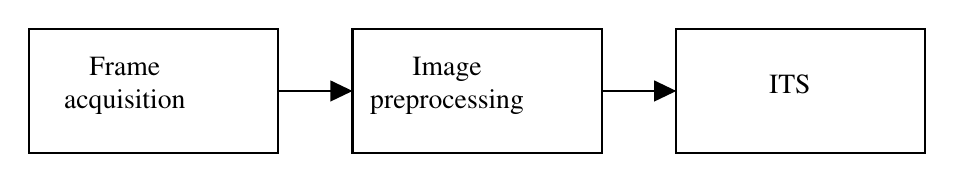
\begin{tikzpicture}[x=0.75pt,y=0.75pt,yscale=-1.2,xscale=1.2]
%uncomment if require: \path (0,300); %set diagram left start at 0, and has height of 300

%Shape: Rectangle [id:dp5311967622096787] 
\draw  [fill={rgb, 255:red, 255; green, 255; blue, 255 }  ,fill opacity=1 ] (20,20) -- (120,20) -- (120,70) -- (20,70) -- cycle ;
%Shape: Rectangle [id:dp07593828947048697] 
\draw  [fill={rgb, 255:red, 255; green, 255; blue, 255 }  ,fill opacity=1 ] (150,20) -- (250,20) -- (250,70) -- (150,70) -- cycle ;
%Shape: Rectangle [id:dp1321828393456428] 
\draw  [fill={rgb, 255:red, 255; green, 255; blue, 255 }  ,fill opacity=1 ] (280,20) -- (380,20) -- (380,70) -- (280,70) -- cycle ;
%Straight Lines [id:da24611526462953326] 
\draw    (120,45) -- (147,45) ;
\draw [shift={(150,45)}, rotate = 180] [fill={rgb, 255:red, 0; green, 0; blue, 0 }  ][line width=0.08]  [draw opacity=0] (8.93,-4.29) -- (0,0) -- (8.93,4.29) -- cycle    ;
%Straight Lines [id:da283033721708871] 
\draw    (250,45) -- (277,45) ;
\draw [shift={(280,45)}, rotate = 180] [fill={rgb, 255:red, 0; green, 0; blue, 0 }  ][line width=0.08]  [draw opacity=0] (8.93,-4.29) -- (0,0) -- (8.93,4.29) -- cycle    ;

% Text Node
\draw (30.67,30.00) node [anchor=north west][inner sep=0.75pt]   [align=left] {\begin{minipage}[lt]{48.000000pt}\setlength\topsep{0pt}
\begin{center}
{\fontfamily{ptm}\selectfont Frame}\\{\fontfamily{ptm}\selectfont  acquisition}
\end{center}

\end{minipage}};
% Text Node
\draw (152,30) node [anchor=north west][inner sep=0.75pt]   [align=left] {\begin{minipage}[lt]{62.482752pt}\setlength\topsep{0pt}
\begin{center}
{\fontfamily{ptm}\selectfont Image}\\{\fontfamily{ptm}\selectfont  preprocessing}
\end{center}

\end{minipage}};
% Text Node
\draw (316,37) node [anchor=north west][inner sep=0.75pt]   [align=left] {{\fontfamily{ptm}\selectfont ITS}};


\end{tikzpicture}

	\caption{Flow Diagram of the proposed method.}
	\label{fig:Scheme}
\end{figure}


The following assumptions are made for the lane detection problem: the lane boundary lines are made of a light color, (e.g., white or yellow); the road has only an ego-lane and lane boundary lines are not covered from other traffic participants. In the following, the three phases reported in Fig.~\ref{fig:Scheme} will be discussed in detail.




\subsection{Frame acquisition}
\label{subsec:Frame_acquisition}


The camera sensor sends~\gls{RGB} format frames to the embedded system. Let $F_i \in \mathbb{R}^{m \times n}$ be the acquired frame channel, where $m\times n$ is the frame size and $i \in \{r,g,b\}$ represent the red, green and blue channel, respectively.

In Figure \ref{fig:road_original} a frame captured from the road scene is presented.

%
\begin{figure}[ht]
	\centering
	\includegraphics[scale=0.55]{figure/Part1/Chapter4/figures/way2.png}
	\caption{Original frame captured from the highway environment.}
	\label{fig:road_original}
\end{figure}

\begin{figure}[ht]
	\centering
	\includegraphics[scale=0.45]{figure/Part1/Chapter4/figures/way3.png}
	\caption{Grayscale conversion and median filtering.}
	\label{fig:road_original_grey}
\end{figure}



\subsection{Image Preprocessing}
\label{subsec:IP}

Usually, an image taken from the highway scenario includes objects that are not significant for lane detection purposes (e.g., trees, clouds, parts of sky, car hood) and these irrelevant objects decrease the overall performance of the algorithm, so in order to clean the original frame from unnecessary information, this image preprocessing step is mandatory. The first step of the image preprocessing consist of a conversion from~\gls{RGB} color model to intensity level frame. Intensity-level conversion is performed by the
weighted sum of~\gls{RGB} frame as follows~\cite{rgbtogray}:
%
\begin{equation}
	I(u,v)=w_r F_r(u,v) + w_g F_g(u,v) + w_b F_b(u,v),
\end{equation}
%
where  $u \in \big\{1, \dots, m\big\}$ and $v \in \big\{1,\dots,n \big\}$ represent the row and column of the selected pixel and $w_r$, $w_g,$ $w_b \in \mathbb{R}$ are the conversion weights of~\gls{RGB} channels. The result of the intensity level conversion can be seen in Figure \ref{fig:road_original_grey}. This conversion reduces the cardinality of the frame and henceforth the computational load placed on the hardware. Furthermore, in order to improve the performances of the lane detection system, a median filter~\cite{gonzalez2002digital} is used, a particular non-linear technique of digital filtering. The application of the filtering stage has two advantages: i) it allows to reduce the noise and ii) it preserves the edges from the captured frame.
Typically, the lane boundary lines are located in the bottom region of a road frame. Taking into account this observation, an isosceles trapezoid~\gls{ROI} operation to restrict the frame information to the road area is performed. Furthermore, shrinking the frame dimensions means that the computational cost of the detection algorithm is further reduced. This procedure is a well known image preprocessing technique as reported in \cite{Kumar2015Stato}. The major base, minor base and the height of the isosceles trapezoid~\gls{ROI} expressed in pixels are $B_{\rm ROI}$, $b_{\rm ROI}$ and $H_{\rm ROI}$, respectively. From now every operation will done on the~\gls{ROI} frame $I_{ \rm ROI} \in \mathbb{R}^{m_{ \rm ROI} \times n_{ \rm ROI}}$, the latter represents an appropriate rectangle matrix where the elements outside the isosceles trapezoid are considered zero.

In Figure~\ref{fig:final_image_preprocessing} the outcome of the image preprocessing  block is shown. 
%
\begin{figure}[ht]
	\centering
	\includegraphics[scale=0.55]{figure/Part1/Chapter4/figures/ROI.png}
	\caption{Frame after the image preprocessing phase. Frame coordinates (Red). Trapezoid major base (Green). Trapezoid minor base (Orange). Trapezoid height (Yellow).}
	\label{fig:final_image_preprocessing}
\end{figure}
%










\subsection{ITS}
\label{subsec:ITS}
The algorithm is in charge to find the pixels belonging to the lane boundary line and is based on an iterative tree search which allows to reduce the lane detection complexity. The concept of this algorithm derives from the idea that the image can be seen as a set of nodes, where these nodes are represented by the pixels. Lane boundaries are solid lines, uniform in color and different from the road color; an edge between the road background and lane boundary lines allows to distinguish the latter from the road in a frame. These structural properties are reformulated from a pixel property point of view.

To explain the~\gls{ITS} algorithm the terms from tree theory are inherited:~\gls{RP} node and~\gls{CP} node. 
%All the above terms have the same meaning of the original tree search theory, but they are applied to the pixel notion. 
In particular, the~\gls{RP} node and~\gls{CP} node contain the intensity level of the pixel. Since the ego-lane has only two lane boundary lines, the algorithm is applied in parallel for each of those.

The first step of the~\gls{ITS} algorithm is to find the first pixel belonging to the lane boundary line, i.e,~\gls{RP}  node. The first~\gls{RP} node is searched among the pixels present in the first row of~\gls{ROI} as reported in Figure~\ref{fig:rootpixel}. Generally, the lane boundary line has a higher intensity level respect to the road; this allows to find the~\gls{RP} node as the pixel having the highest intensity level. In Figure~\ref{fig:rootframe} the intensity level profile regarding the first row of the~\gls{ROI} is shown, where two peaks are distinguishable that represents the two~\gls{RP}  nodes for the two lane boundary lines.

\begin{figure}[ht]
	\centering
	\includegraphics[scale=0.55]{figure/Part1/Chapter4/figures/roi.png}
	\caption{Finding the~\gls{RP} nodes. First pixel row~\gls{ROI} (Red).~\gls{RP} nodes (Blue). }
	\label{fig:rootpixel}
\end{figure}

\begin{figure} [ht]
	\centering
	\includegraphics[scale=0.3]{figure/Part1/Chapter4/figures/plot.png}
	\caption{Intensity level first row~\gls{ROI}.}
	\label{fig:rootframe}
\end{figure} 



Once the first~\gls{RP}  node is found, a number $N_c$ of~\gls{CP}  nodes are inspected to find another pixel belonging to the lane boundary line on the above row of $I_{\rm ROI}$. The choice is based on the following score function $J$ which measures the score obtained from all the~\gls{CP}  nodes:
%
\begin{equation} \label{eq:J}
		J(u,v)= \alpha I_{\rm ROI}(u,v) - \beta \mid v - v_r \mid +
		-\gamma \mid I_{\rm ROI}(u,v)-I_{\rm ROI}(u_r,v_r) \mid,
\end{equation}
%
where $u,v$  $\big(u_r,v_r\big)$ represent the row and column of~\gls{CP} node \mbox{(\gls{RP} node)}, respectively. The parameters $\alpha$, $\beta$ and $\gamma$ are used to weight the contributes coming from the three addends. The first addend is the intensity level of the~\gls{CP} node, the second and third addends are the distance and the color dissimilarity between the~\gls{CP} node and root pixel node, respectively. 
The first term encourage the choice of brighter pixels; the second term penalizes the pixels that are farther from the root pixel, while the third term is added to encourage the uniformity of intensity between the~\gls{RP} and~\gls{CP}.
Once the functional scores are calculated for each~\gls{CP} node, the one with highest score become the new~\gls{RP} node. Finally the pair $\big(u_r, v_r \big)$ is saved into a memory buffer. The algorithm is iterated until the~\gls{RP} node row reaches the height $H_{\rm ROI}$ of the~\gls{ROI}. In Algorithm~\ref{alg:ITSAlg} the entire procedure is reported.

\begin{algorithm}
	\caption{ITS}\label{alg:ITSAlg}
	\begin{algorithmic}[1]
		\State  $u_r \gets 1$
		\State   $v_r \gets \text{FindRoot}(u_r)$
		\State $LaneSet \gets (u_r,v_r) $
		\While{$u_r \leq H_{ \rm ROI}$}
		\For{$v \in \big\{ v_r-\frac{N_c}{2},\dots,v_r+\frac{N_c}{2}\big\} $}
		\State \text{score function in \eqref{eq:J}.}
		\EndFor
		\State $v_r = \argmax_v \; J(u_r,v)$
		\State $LaneSet \gets (u_r,v_r) $
		\State  $u_r \gets u_r +1$
		\EndWhile
		\State \Return $LaneSet$
	\end{algorithmic}
\end{algorithm} 


\noindent A illustration of the proposed algorithm is presented in Figure~\ref{fig:ITS_double}. In  Fig.~\ref{fig:u1} the~\gls{RP} node is represented with the yellow square. This pixel has been chosen as the pixel with the maximum intensity between the ones in the first row of~\gls{ROI}. The green squares represent the~\gls{CP} nodes, and for each one of them, the score function presented in~\eqref{eq:J} is evaluated. Then, the new~\gls{RP} node will be chosen among the~\gls{CP} nodes as the one that maximise the score function (Fig.~\ref{fig:u2}).

\begin{figure}[ht]
	\begin{subfigure}[b]{\textwidth}
		\centering
		


\tikzset{every picture/.style={line width=0.75pt}} %set default line width to 0.75pt        

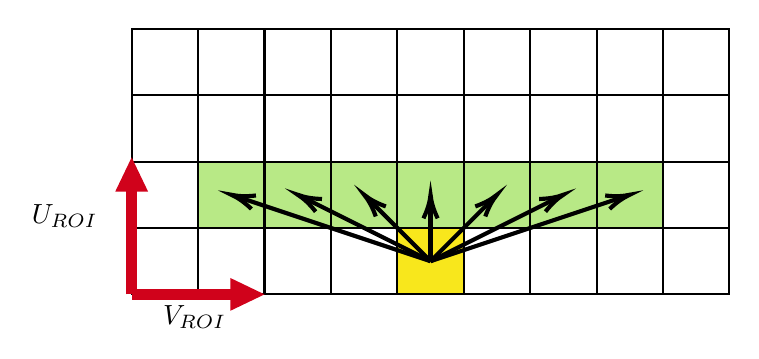
\begin{tikzpicture}[x=0.75pt,y=0.75pt,yscale=-0.8,xscale=0.8]
%uncomment if require: \path (0,300); %set diagram left start at 0, and has height of 300

%Shape: Rectangle [id:dp37479279946268607] 
\draw   (157,53) -- (197,53) -- (197,93) -- (157,93) -- cycle ;
%Shape: Rectangle [id:dp9386900567441059] 
\draw   (197,53) -- (237,53) -- (237,93) -- (197,93) -- cycle ;
%Shape: Rectangle [id:dp40563047766175897] 
\draw   (237,53) -- (277,53) -- (277,93) -- (237,93) -- cycle ;
%Shape: Rectangle [id:dp5068636395583868] 
\draw   (277,53) -- (317,53) -- (317,93) -- (277,93) -- cycle ;
%Shape: Rectangle [id:dp8547935475054569] 
\draw   (317,53) -- (357,53) -- (357,93) -- (317,93) -- cycle ;
%Shape: Rectangle [id:dp7875634623224428] 
\draw   (357,53) -- (397,53) -- (397,93) -- (357,93) -- cycle ;
%Shape: Rectangle [id:dp48004515510156187] 
\draw   (397,53) -- (437,53) -- (437,93) -- (397,93) -- cycle ;
%Shape: Rectangle [id:dp24690344103074247] 
\draw   (477,53) -- (517,53) -- (517,93) -- (477,93) -- cycle ;
%Shape: Rectangle [id:dp92756370861019] 
\draw   (437,53) -- (477,53) -- (477,93) -- (437,93) -- cycle ;
%Shape: Rectangle [id:dp27395603578063277] 
\draw   (157,93) -- (197,93) -- (197,133) -- (157,133) -- cycle ;
%Shape: Rectangle [id:dp1408582450054794] 
\draw   (197,93) -- (237,93) -- (237,133) -- (197,133) -- cycle ;
%Shape: Rectangle [id:dp2887808288270002] 
\draw   (237,93) -- (277,93) -- (277,133) -- (237,133) -- cycle ;
%Shape: Rectangle [id:dp33037939362347357] 
\draw   (277,93) -- (317,93) -- (317,133) -- (277,133) -- cycle ;
%Shape: Rectangle [id:dp3538768626341806] 
\draw   (317,93) -- (357,93) -- (357,133) -- (317,133) -- cycle ;
%Shape: Rectangle [id:dp9814839313159069] 
\draw   (357,93) -- (397,93) -- (397,133) -- (357,133) -- cycle ;
%Shape: Rectangle [id:dp12604922129270824] 
\draw   (397,93) -- (437,93) -- (437,133) -- (397,133) -- cycle ;
%Shape: Rectangle [id:dp3422014175969996] 
\draw   (477,93) -- (517,93) -- (517,133) -- (477,133) -- cycle ;
%Shape: Rectangle [id:dp7920304225353518] 
\draw   (437,93) -- (477,93) -- (477,133) -- (437,133) -- cycle ;
%Shape: Rectangle [id:dp18661999462756818] 
\draw   (157,133) -- (197,133) -- (197,173) -- (157,173) -- cycle ;
%Shape: Rectangle [id:dp18791201855733464] 
\draw  [fill={rgb, 255:red, 184; green, 233; blue, 134 }  ,fill opacity=1 ] (197,133) -- (237,133) -- (237,173) -- (197,173) -- cycle ;
%Shape: Rectangle [id:dp5629889443468381] 
\draw  [fill={rgb, 255:red, 184; green, 233; blue, 134 }  ,fill opacity=1 ] (237,133) -- (277,133) -- (277,173) -- (237,173) -- cycle ;
%Shape: Rectangle [id:dp503276244238676] 
\draw  [fill={rgb, 255:red, 184; green, 233; blue, 134 }  ,fill opacity=1 ] (277,133) -- (317,133) -- (317,173) -- (277,173) -- cycle ;
%Shape: Rectangle [id:dp4070792760484063] 
\draw  [fill={rgb, 255:red, 184; green, 233; blue, 134 }  ,fill opacity=1 ] (317,133) -- (357,133) -- (357,173) -- (317,173) -- cycle ;
%Shape: Rectangle [id:dp2619995679469691] 
\draw  [fill={rgb, 255:red, 184; green, 233; blue, 134 }  ,fill opacity=1 ] (357,133) -- (397,133) -- (397,173) -- (357,173) -- cycle ;
%Shape: Rectangle [id:dp8991355658683184] 
\draw  [fill={rgb, 255:red, 184; green, 233; blue, 134 }  ,fill opacity=1 ] (397,133) -- (437,133) -- (437,173) -- (397,173) -- cycle ;
%Shape: Rectangle [id:dp03123946616100537] 
\draw   (477,133) -- (517,133) -- (517,173) -- (477,173) -- cycle ;
%Shape: Rectangle [id:dp6406090567697098] 
\draw  [fill={rgb, 255:red, 184; green, 233; blue, 134 }  ,fill opacity=1 ] (437,133) -- (477,133) -- (477,173) -- (437,173) -- cycle ;
%Shape: Rectangle [id:dp923072610195202] 
\draw   (157,173) -- (197,173) -- (197,213) -- (157,213) -- cycle ;
%Shape: Rectangle [id:dp40649773535656464] 
\draw   (197,173) -- (237,173) -- (237,213) -- (197,213) -- cycle ;
%Shape: Rectangle [id:dp05637699840141841] 
\draw   (237,173) -- (277,173) -- (277,213) -- (237,213) -- cycle ;
%Shape: Rectangle [id:dp10908609515836498] 
\draw   (277,173) -- (317,173) -- (317,213) -- (277,213) -- cycle ;
%Shape: Rectangle [id:dp1978162709414546] 
\draw  [fill={rgb, 255:red, 248; green, 231; blue, 28 }  ,fill opacity=1 ] (317,173) -- (357,173) -- (357,213) -- (317,213) -- cycle ;
%Shape: Rectangle [id:dp09177043950937769] 
\draw   (357,173) -- (397,173) -- (397,213) -- (357,213) -- cycle ;
%Shape: Rectangle [id:dp840673321356215] 
\draw   (397,173) -- (437,173) -- (437,213) -- (397,213) -- cycle ;
%Shape: Rectangle [id:dp4916817832684255] 
\draw   (477,173) -- (517,173) -- (517,213) -- (477,213) -- cycle ;
%Shape: Rectangle [id:dp73827422693894] 
\draw   (437,173) -- (477,173) -- (477,213) -- (437,213) -- cycle ;
%Straight Lines [id:da8560297776013615] 
\draw [line width=1.5]    (337,193) -- (219.85,153.95) ;
\draw [shift={(217,153)}, rotate = 378.43] [color={rgb, 255:red, 0; green, 0; blue, 0 }  ][line width=1.5]    (14.21,-4.28) .. controls (9.04,-1.82) and (4.3,-0.39) .. (0,0) .. controls (4.3,0.39) and (9.04,1.82) .. (14.21,4.28)   ;
%Straight Lines [id:da27817194509681964] 
\draw [line width=1.5]    (337,193) -- (259.68,154.34) ;
\draw [shift={(257,153)}, rotate = 386.57] [color={rgb, 255:red, 0; green, 0; blue, 0 }  ][line width=1.5]    (14.21,-4.28) .. controls (9.04,-1.82) and (4.3,-0.39) .. (0,0) .. controls (4.3,0.39) and (9.04,1.82) .. (14.21,4.28)   ;
%Straight Lines [id:da07123008278456933] 
\draw [line width=1.5]    (337,193) -- (299.12,155.12) ;
\draw [shift={(297,153)}, rotate = 405] [color={rgb, 255:red, 0; green, 0; blue, 0 }  ][line width=1.5]    (14.21,-4.28) .. controls (9.04,-1.82) and (4.3,-0.39) .. (0,0) .. controls (4.3,0.39) and (9.04,1.82) .. (14.21,4.28)   ;
%Straight Lines [id:da81869629277768] 
\draw [line width=1.5]    (337,193) -- (337,156) ;
\draw [shift={(337,153)}, rotate = 450] [color={rgb, 255:red, 0; green, 0; blue, 0 }  ][line width=1.5]    (14.21,-4.28) .. controls (9.04,-1.82) and (4.3,-0.39) .. (0,0) .. controls (4.3,0.39) and (9.04,1.82) .. (14.21,4.28)   ;
%Straight Lines [id:da7756735099229475] 
\draw [line width=1.5]    (337,193) -- (374.88,155.12) ;
\draw [shift={(377,153)}, rotate = 495] [color={rgb, 255:red, 0; green, 0; blue, 0 }  ][line width=1.5]    (14.21,-4.28) .. controls (9.04,-1.82) and (4.3,-0.39) .. (0,0) .. controls (4.3,0.39) and (9.04,1.82) .. (14.21,4.28)   ;
%Straight Lines [id:da07783001016646374] 
\draw [line width=1.5]    (337,193) -- (414.32,154.34) ;
\draw [shift={(417,153)}, rotate = 513.4300000000001] [color={rgb, 255:red, 0; green, 0; blue, 0 }  ][line width=1.5]    (14.21,-4.28) .. controls (9.04,-1.82) and (4.3,-0.39) .. (0,0) .. controls (4.3,0.39) and (9.04,1.82) .. (14.21,4.28)   ;
%Straight Lines [id:da5414037753227225] 
\draw [line width=1.5]    (337,193) -- (454.15,153.95) ;
\draw [shift={(457,153)}, rotate = 521.5699999999999] [color={rgb, 255:red, 0; green, 0; blue, 0 }  ][line width=1.5]    (14.21,-4.28) .. controls (9.04,-1.82) and (4.3,-0.39) .. (0,0) .. controls (4.3,0.39) and (9.04,1.82) .. (14.21,4.28)   ;
%Straight Lines [id:da8047399591588045] 
\draw [color={rgb, 255:red, 208; green, 2; blue, 27 }  ,draw opacity=1 ][line width=3.75]    (157,213) -- (157,137.5) ;
\draw [shift={(157,130.5)}, rotate = 450] [fill={rgb, 255:red, 208; green, 2; blue, 27 }  ,fill opacity=1 ][line width=0.08]  [draw opacity=0] (20.54,-9.87) -- (0,0) -- (20.54,9.87) -- cycle    ;
%Straight Lines [id:da39334795544652645] 
\draw [color={rgb, 255:red, 208; green, 2; blue, 27 }  ,draw opacity=1 ][line width=3.75]    (157,213) -- (230,213) ;
\draw [shift={(237,213)}, rotate = 180] [fill={rgb, 255:red, 208; green, 2; blue, 27 }  ,fill opacity=1 ][line width=0.08]  [draw opacity=0] (20.54,-9.87) -- (0,0) -- (20.54,9.87) -- cycle    ;

% Text Node
\draw (95,157) node [anchor=north west][inner sep=0.75pt]    {$U_{ROI}$};
% Text Node
\draw (174,218) node [anchor=north west][inner sep=0.75pt]    {$V_{ROI}$};


\end{tikzpicture}

		\caption{}
		\label{fig:u1}
	\end{subfigure}
	\\[3ex]
	\begin{subfigure}[b]{\textwidth}
		\centering
		


\tikzset{every picture/.style={line width=0.75pt}} %set default line width to 0.75pt        

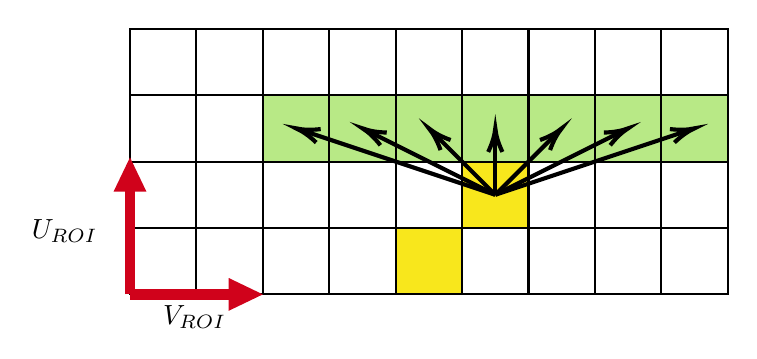
\begin{tikzpicture}[x=0.75pt,y=0.75pt,yscale=-0.8,xscale=0.8]
%uncomment if require: \path (0,300); %set diagram left start at 0, and has height of 300

%Shape: Rectangle [id:dp44188910505312085] 
\draw   (196,145) -- (236,145) -- (236,185) -- (196,185) -- cycle ;
%Shape: Rectangle [id:dp17982965297494968] 
\draw   (236,145) -- (276,145) -- (276,185) -- (236,185) -- cycle ;
%Shape: Rectangle [id:dp22515587821006955] 
\draw   (276,145) -- (316,145) -- (316,185) -- (276,185) -- cycle ;
%Shape: Rectangle [id:dp11801076383471742] 
\draw  [fill={rgb, 255:red, 248; green, 231; blue, 28 }  ,fill opacity=1 ] (316,145) -- (356,145) -- (356,185) -- (316,185) -- cycle ;
%Shape: Rectangle [id:dp9089046489603911] 
\draw   (356,145) -- (396,145) -- (396,185) -- (356,185) -- cycle ;
%Shape: Rectangle [id:dp7896999403341205] 
\draw   (396,145) -- (436,145) -- (436,185) -- (396,185) -- cycle ;
%Shape: Rectangle [id:dp9713409962967257] 
\draw   (436,145) -- (476,145) -- (476,185) -- (436,185) -- cycle ;
%Shape: Rectangle [id:dp014859460901382793] 
\draw   (156,145) -- (196,145) -- (196,185) -- (156,185) -- cycle ;
%Shape: Rectangle [id:dp9620038332096106] 
\draw   (476,145) -- (516,145) -- (516,185) -- (476,185) -- cycle ;
%Shape: Rectangle [id:dp9318475849101779] 
\draw   (196,25) -- (236,25) -- (236,65) -- (196,65) -- cycle ;
%Shape: Rectangle [id:dp23554291041537723] 
\draw   (236,25) -- (276,25) -- (276,65) -- (236,65) -- cycle ;
%Shape: Rectangle [id:dp6788071985488238] 
\draw   (276,25) -- (316,25) -- (316,65) -- (276,65) -- cycle ;
%Shape: Rectangle [id:dp6202713322137914] 
\draw   (316,25) -- (356,25) -- (356,65) -- (316,65) -- cycle ;
%Shape: Rectangle [id:dp771670694696643] 
\draw   (356,25) -- (396,25) -- (396,65) -- (356,65) -- cycle ;
%Shape: Rectangle [id:dp48752893858306945] 
\draw   (396,25) -- (436,25) -- (436,65) -- (396,65) -- cycle ;
%Shape: Rectangle [id:dp8558160524482463] 
\draw   (436,25) -- (476,25) -- (476,65) -- (436,65) -- cycle ;
%Shape: Rectangle [id:dp9591030266017664] 
\draw   (156,25) -- (196,25) -- (196,65) -- (156,65) -- cycle ;
%Shape: Rectangle [id:dp40356174570980485] 
\draw   (476,25) -- (516,25) -- (516,65) -- (476,65) -- cycle ;
%Shape: Rectangle [id:dp47130309531175807] 
\draw   (196,65) -- (236,65) -- (236,105) -- (196,105) -- cycle ;
%Shape: Rectangle [id:dp4748802662239511] 
\draw  [fill={rgb, 255:red, 184; green, 233; blue, 134 }  ,fill opacity=1 ] (236,65) -- (276,65) -- (276,105) -- (236,105) -- cycle ;
%Shape: Rectangle [id:dp11159600208179388] 
\draw  [fill={rgb, 255:red, 184; green, 233; blue, 134 }  ,fill opacity=1 ] (276,65) -- (316,65) -- (316,105) -- (276,105) -- cycle ;
%Shape: Rectangle [id:dp2885743588567362] 
\draw  [fill={rgb, 255:red, 184; green, 233; blue, 134 }  ,fill opacity=1 ] (316,65) -- (356,65) -- (356,105) -- (316,105) -- cycle ;
%Shape: Rectangle [id:dp8432572496496091] 
\draw  [fill={rgb, 255:red, 184; green, 233; blue, 134 }  ,fill opacity=1 ] (356,65) -- (396,65) -- (396,105) -- (356,105) -- cycle ;
%Shape: Rectangle [id:dp8352049942769133] 
\draw  [fill={rgb, 255:red, 184; green, 233; blue, 134 }  ,fill opacity=1 ] (396,65) -- (436,65) -- (436,105) -- (396,105) -- cycle ;
%Shape: Rectangle [id:dp8429572386016915] 
\draw  [fill={rgb, 255:red, 184; green, 233; blue, 134 }  ,fill opacity=1 ] (436,65) -- (476,65) -- (476,105) -- (436,105) -- cycle ;
%Shape: Rectangle [id:dp26640609195013454] 
\draw   (156,65) -- (196,65) -- (196,105) -- (156,105) -- cycle ;
%Shape: Rectangle [id:dp07095927085369014] 
\draw  [fill={rgb, 255:red, 184; green, 233; blue, 134 }  ,fill opacity=1 ] (476,65) -- (516,65) -- (516,105) -- (476,105) -- cycle ;
%Shape: Rectangle [id:dp4884033403677166] 
\draw   (196,105) -- (236,105) -- (236,145) -- (196,145) -- cycle ;
%Shape: Rectangle [id:dp9615981099361754] 
\draw   (236,105) -- (276,105) -- (276,145) -- (236,145) -- cycle ;
%Shape: Rectangle [id:dp7798644660619822] 
\draw   (276,105) -- (316,105) -- (316,145) -- (276,145) -- cycle ;
%Shape: Rectangle [id:dp8219025004188054] 
\draw   (316,105) -- (356,105) -- (356,145) -- (316,145) -- cycle ;
%Shape: Rectangle [id:dp06887054649368096] 
\draw  [fill={rgb, 255:red, 248; green, 231; blue, 28 }  ,fill opacity=1 ] (356,105) -- (396,105) -- (396,145) -- (356,145) -- cycle ;
%Shape: Rectangle [id:dp6604033014043791] 
\draw   (396,105) -- (436,105) -- (436,145) -- (396,145) -- cycle ;
%Shape: Rectangle [id:dp6485467100115199] 
\draw   (436,105) -- (476,105) -- (476,145) -- (436,145) -- cycle ;
%Shape: Rectangle [id:dp8619997043000098] 
\draw   (156,105) -- (196,105) -- (196,145) -- (156,145) -- cycle ;
%Shape: Rectangle [id:dp610853992697381] 
\draw   (476,105) -- (516,105) -- (516,145) -- (476,145) -- cycle ;
%Straight Lines [id:da20862453693670302] 
\draw [line width=1.5]    (376,125) -- (258.85,85.95) ;
\draw [shift={(256,85)}, rotate = 378.43] [color={rgb, 255:red, 0; green, 0; blue, 0 }  ][line width=1.5]    (14.21,-4.28) .. controls (9.04,-1.82) and (4.3,-0.39) .. (0,0) .. controls (4.3,0.39) and (9.04,1.82) .. (14.21,4.28)   ;
%Straight Lines [id:da23890585644446216] 
\draw [line width=1.5]    (376,125) -- (298.68,86.34) ;
\draw [shift={(296,85)}, rotate = 386.57] [color={rgb, 255:red, 0; green, 0; blue, 0 }  ][line width=1.5]    (14.21,-4.28) .. controls (9.04,-1.82) and (4.3,-0.39) .. (0,0) .. controls (4.3,0.39) and (9.04,1.82) .. (14.21,4.28)   ;
%Straight Lines [id:da8795814409036085] 
\draw [line width=1.5]    (376,125) -- (338.12,87.12) ;
\draw [shift={(336,85)}, rotate = 405] [color={rgb, 255:red, 0; green, 0; blue, 0 }  ][line width=1.5]    (14.21,-4.28) .. controls (9.04,-1.82) and (4.3,-0.39) .. (0,0) .. controls (4.3,0.39) and (9.04,1.82) .. (14.21,4.28)   ;
%Straight Lines [id:da3518187431990738] 
\draw [line width=1.5]    (376,125) -- (376,88) ;
\draw [shift={(376,85)}, rotate = 450] [color={rgb, 255:red, 0; green, 0; blue, 0 }  ][line width=1.5]    (14.21,-4.28) .. controls (9.04,-1.82) and (4.3,-0.39) .. (0,0) .. controls (4.3,0.39) and (9.04,1.82) .. (14.21,4.28)   ;
%Straight Lines [id:da6169575633471645] 
\draw [line width=1.5]    (376,125) -- (413.88,87.12) ;
\draw [shift={(416,85)}, rotate = 495] [color={rgb, 255:red, 0; green, 0; blue, 0 }  ][line width=1.5]    (14.21,-4.28) .. controls (9.04,-1.82) and (4.3,-0.39) .. (0,0) .. controls (4.3,0.39) and (9.04,1.82) .. (14.21,4.28)   ;
%Straight Lines [id:da8677184701710603] 
\draw [line width=1.5]    (376,125) -- (453.32,86.34) ;
\draw [shift={(456,85)}, rotate = 513.4300000000001] [color={rgb, 255:red, 0; green, 0; blue, 0 }  ][line width=1.5]    (14.21,-4.28) .. controls (9.04,-1.82) and (4.3,-0.39) .. (0,0) .. controls (4.3,0.39) and (9.04,1.82) .. (14.21,4.28)   ;
%Straight Lines [id:da6146087490578516] 
\draw [line width=1.5]    (376,125) -- (493.15,85.95) ;
\draw [shift={(496,85)}, rotate = 521.5699999999999] [color={rgb, 255:red, 0; green, 0; blue, 0 }  ][line width=1.5]    (14.21,-4.28) .. controls (9.04,-1.82) and (4.3,-0.39) .. (0,0) .. controls (4.3,0.39) and (9.04,1.82) .. (14.21,4.28)   ;
%Straight Lines [id:da5907668863809314] 
\draw [color={rgb, 255:red, 208; green, 2; blue, 27 }  ,draw opacity=1 ][line width=3.75]    (156,185) -- (156,109.5) ;
\draw [shift={(156,102.5)}, rotate = 450] [fill={rgb, 255:red, 208; green, 2; blue, 27 }  ,fill opacity=1 ][line width=0.08]  [draw opacity=0] (20.54,-9.87) -- (0,0) -- (20.54,9.87) -- cycle    ;
%Straight Lines [id:da013929014083935432] 
\draw [color={rgb, 255:red, 208; green, 2; blue, 27 }  ,draw opacity=1 ][line width=3.75]    (156,185) -- (229,185) ;
\draw [shift={(236,185)}, rotate = 180] [fill={rgb, 255:red, 208; green, 2; blue, 27 }  ,fill opacity=1 ][line width=0.08]  [draw opacity=0] (20.54,-9.87) -- (0,0) -- (20.54,9.87) -- cycle    ;

% Text Node
\draw (95,138) node [anchor=north west][inner sep=0.75pt]    {$U_{ROI}$};
% Text Node
\draw (174,190) node [anchor=north west][inner sep=0.75pt]    {$V_{ROI}$};


\end{tikzpicture}
		\caption{}
		\label{fig:u2}
	\end{subfigure}
	\caption{Illustration of the algorithm. First iteration (Fig.~\ref{fig:u1}). Second iteration (Fig.~\ref{fig:u2}). Green and Yellow colors represent~\gls{CP} node and~\gls{RP}  node, respectively.}
	\label{fig:ITS_double}
\end{figure}


The~\gls{ITS} algorithm implemented has time complexity $O\big((N_c+1) H_{\rm ROI}\big)$ that is two order lower than~\gls{HT} that is $O\big((m n)^4\big)$~\cite{albanesi1991time}, where $m$ and $n$ are the width and the height of the original frame. The minor time complexity permits implementation on embedded systems. Furthermore, the parallelization of the algorithm is possible using a multicore CPU, Graphics Processing Unit or Field-Programmable Gate Array in order to further reduce the computation time. 

\section{Experimental Setup}
\label{sec:Experimental results}

To evaluate the timing performance of the proposed~\gls{ITS} algorithm, a series of real-world road sequences with different illumination conditions are collected. The data sets cover three kinds of road scenarios, such as: (i) night scenario, (ii) daytime scenario, and (iii) the fluctuating illumination scenario. The experimental setup used for the tests is shown in Figure~\ref{fig:setup}. The main components used are two low-cost hardware devices, which will be described below.

\begin{figure}[ht]
	\centering
	\includegraphics[scale=0.4]{figure/Part1/Chapter4/figures/setup.jpg}
	\caption{Hardware setup.}
	\label{fig:setup}
\end{figure}

The proposed algorithm is implemented using Python $3.6$ and OpenCV library on a Nvidia Jetson Nano platform (Figure), an embedded system composed of quadcore Arm $57$ CPU with a clock frequency of~\SI{1.43}{\GHz} and~\SI{4}{\giga \byte} of RAM. A camera sensor Sony IMX$219$PQH$5$-C (Figure) is used and mounted on the car hood. The camera is a CMOS active pixel type image sensor with a square pixel array and $8.08$ Million of pixels. In addition to being a low-cost experimental setup, it also has a total power consumption of \SI{5}{\watt} thus making the proposed system an appealing solution for low power applications. 


\subsection{Results}


Furthermore, a comparison between computation times of the proposed algorithm and the other state of the art lane detection algorithm has been carried out. The~\gls{ITS} algorithm takes 
%has a computation time of 
\SI{30}{\milli \second} to detect both lanes, this means it can achieve 33.3 Frame Per Second (FPS).
In~\cite{aly2008real} and~\cite{liu2013lane}, the computation time of the algorithms are \SI{20}{\milli\second} and \SI{200}{\milli\second}, respectively; here more powerful hardware was used with a lower frame resolution thus reducing the overall computational effort. The proposed algorithm shows reasonable computation times with a less expensive hardware; furthermore, it allows to parallelize the detection of multiple lane boundaries on a multicore system. 

Figure~\ref{fig:ITS_results} presents results of applying the proposed algorithm to scenarios with different illumination conditions. In particular, three scenarios are reported to appreciate the effectiveness of the proposed method: clear sky, night road and different tunnel with multiple illuminations.  

\begin{figure}[ht]
	\centering
	\includegraphics[scale=0.45]{figure/Part1/Chapter4/figures/test_final_letter.png}
	\caption{Results in different light scenarios. clear sky  (a); under different tunnels with different luminosity (b)-(e); night road (f).}
	\label{fig:ITS_results}
\end{figure}

By observing the results presented in Fig.~\ref{fig:ITS_results} it is possible to notice that the proposed algorithm manages to precisely track the road lane in all the conditions tested. When there is a change in brightness, for example when the car enters a tunnel, it is possible to notice a minor deviation between the effective position of the lane and the one tracked by the algorithm. Nevertheless, the line detection is still carried out. Good performances are also observed in the condition of scarce brightness, where the tracking is still precise. 
Generally speaking, by taking into account all scenarios, the proposed method manages to precisely detect a lane, both when there is good brightness and when there is not.

\newpage
\newpage
\section{Chapter Summary}



In concluding this chapter, we have demonstrated the effectiveness of the Iterative Tree Search (ITS) algorithm in the realm of autonomous driving, specifically addressing the critical aspect of lane detection. Through rigorous testing and evaluation under diverse conditions, the ITS algorithm has proven to be a robust and reliable solution, offering significant advantages over traditional methods in terms of computational efficiency and adaptability to varying environmental conditions.

The success of the ITS algorithm underscores the potential for significant advancements in real-time lane detection technologies, contributing to safer and more reliable autonomous driving systems. By optimizing for both accuracy and computational resourcefulness, the algorithm ensures its applicability across a wide range of automotive platforms, from high-end autonomous vehicles to more accessible driver-assistance systems.



